\documentclass{article}
\usepackage[margin=1in]{geometry}
\usepackage{amsmath,amsthm,amssymb}
\usepackage{bbm,enumerate,mathtools}
\usepackage{tikz,pgfplots}
\usepackage{chessboard}
\usepackage[hidelinks]{hyperref}
\usepackage{multicol} % Problem 35

\newenvironment{question}{\begin{trivlist}\item[\textbf{Question.}]}{\end{trivlist}}
\newenvironment{note}{\begin{trivlist}\item[\textbf{Note.}]}{\end{trivlist}}
\newenvironment{references}{\begin{trivlist}\item[\textbf{References.}]}{\end{trivlist}}
\newenvironment{related}{\begin{trivlist}\item[\textbf{Related.}]\end{trivlist}\begin{enumerate}}{\end{enumerate}}


\begin{document}
\rating{2}{2}
Let $f_{n,m}: [n] \rightarrow [m]$ be a uniformly random function.
Consider the convex hull around $\{(1, f(1)), \hdots (n, f(n))\}$
\begin{figure}[!h]
  \centering
  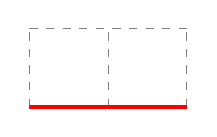
\begin{tikzpicture}
    \draw[gray, dashed] (0, 0) grid (2, 1);
    \draw[red, very thick] (0, 0) -- (1, 0) -- (2, 0);
  \end{tikzpicture}\hspace{0.5cm}
  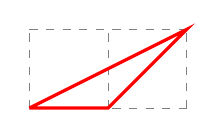
\begin{tikzpicture}
    \draw[gray, dashed] (0, 0) grid (2, 1);
    \draw[red, very thick] (0, 0) -- (1, 0) -- (2, 1) -- (0, 0);
  \end{tikzpicture}\hspace{0.5cm}
  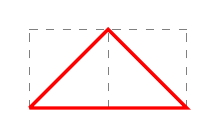
\begin{tikzpicture}
    \draw[gray, dashed] (0, 0) grid (2, 1);
    \draw[red, very thick] (0, 0) -- (1, 1) -- (2, 0) -- (0, 0);
  \end{tikzpicture}\hspace{0.5cm}
  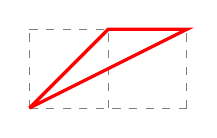
\begin{tikzpicture}
    \draw[gray, dashed] (0, 0) grid (2, 1);
    \draw[red, very thick] (0, 0) -- (1, 1) -- (2, 1) -- (0, 0);
  \end{tikzpicture}\hspace{0.5cm}\\~\\
  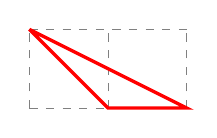
\begin{tikzpicture}
    \draw[gray, dashed] (0, 0) grid (2, 1);
    \draw[red, very thick] (0, 1) -- (1, 0) -- (2, 0) -- (0, 1);
  \end{tikzpicture}\hspace{0.5cm}
  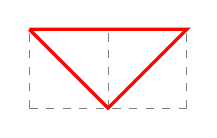
\begin{tikzpicture}
    \draw[gray, dashed] (0, 0) grid (2, 1);
    \draw[red, very thick] (0, 1) -- (1, 0) -- (2, 1) -- (0, 1);
  \end{tikzpicture}\hspace{0.5cm}
  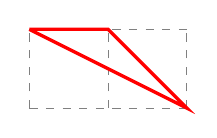
\begin{tikzpicture}
    \draw[gray, dashed] (0, 0) grid (2, 1);
    \draw[red, very thick] (0, 1) -- (1, 1) -- (2, 0) -- (0, 1);
  \end{tikzpicture}\hspace{0.5cm}
  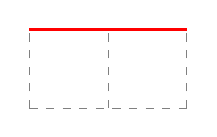
\begin{tikzpicture}
    \draw[gray, dashed] (0, 0) grid (2, 1);
    \draw[red, very thick] (0, 1) -- (1, 1) -- (2, 1);
  \end{tikzpicture}

  \caption{Examples of $f_{3,2}$. Here the expected number of vertices on a convex hull is $2.75$}
\end{figure}

\begin{question}
  What is the probability of seeing a $k$-gon (for some fixed $k$), when given
  a uniformly random function $f_{n,m}$?
\end{question}

\begin{related}
  \item What if $f_{n,n}$ is restricted to be a permutation?
  \item What if $f_{n,m}$ is injective?
\end{related}
\end{document}
